\documentclass[10pt,twocolumn,letterpaper]{article}

\usepackage{cvpr}
\usepackage{times}
\usepackage{epsfig}
\usepackage{graphicx}
\usepackage{amsmath}
\usepackage{amssymb}
\usepackage{pifont}
\usepackage{multirow}

\usepackage[breaklinks=true,bookmarks=false]{hyperref}

\cvprfinalcopy

\def\httilde{\mbox{\tt\raisebox{-.5ex}{\symbol{126}}}}

\begin{document}

%%%%%%%%% TITLE
\title{MiniPlaces Challenge: AhHeyNet}

\author{Christina Sun\\
6.869\\
{\tt\small sunc@mit.edu}
\and
Larry Zhang\\
6.869\\
{\tt\small larryq@mit.edu}
}

\maketitle

\begin{abstract}
   We study three established convolutional neural nets for the task of identifying scene categories in the MiniPlaces dataset. We then experiment with various modifications to these models with the goal of improving their top-5 accuracy. We investigate data augmentation through subsampling and flipping, including modules from other model architectures, and averaging predictions across different models. Our final model achieves a score of 0.752.
\end{abstract}

\section{Introduction}

The development of deep learning methods, particularly the use of convolutional neural networks, has greatly increased performance in computer vision classification tasks. In addition, the training datasets required to perform these tasks have become quite large, containing millions of images.

In this paper, we tackle the MiniPlaces Challenge, in which the goal is to identify the scene category depicted in a photograph. The MiniPlaces dataset is a subset of the Places2 dataset~\cite{places2}, and contains 100,000 training, 10,000 validation, and 10,000 test images, all of size 128 $\times$ 128. Images in the training and validation sets are each labeled with one of 100 scene categories. Figure~\ref{fig:dataset} shows two sample training images.

\begin{figure}[ht]
\centering
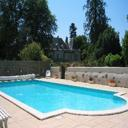
\includegraphics[width=0.49\linewidth]{imgs/swimmingpool.jpg}
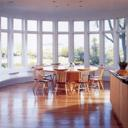
\includegraphics[width=0.49\linewidth]{imgs/diningroom.jpg}
\caption{Two example images from the MiniPlaces dataset. The corresponding scene category labels are \texttt{swimming pool} (left) and \texttt{dining room} (right).}
\label{fig:dataset}
\end{figure}

In order to classify the images in the MiniPlaces dataset, we first explore three existing base architectures: AlexNet~\cite{alexnet}, VGG16, and VGG19~\cite{vgg}. We describe modifications that we performed to each model, along with the hybrid VGG19-AlexNet model used in the final test set predictions submitted to the class leaderboard. This hybrid model achieves a top-5 test accuracy of 0.752.

\subsection{Division of Work}

Together, we pair-coded a baseline infrastructure using the Python Keras library~\cite{keras}. This pipeline handled preprocessing data, training and validating the model, as well as predicting labels for the test set. Initially, we also worked together to implement a version of AlexNet using Keras. Later, to parallelize trying different modifications, Larry focused on modifications within a single model (augmenting inputs), while Christina focused on combining predictions from different models (averaging predictions). The details of these modifications are discussed in Section~\ref{sec:approach}. Finally, we wrote this report together.


\section{Approach}\label{sec:approach}
Due to computational and monetary limitations of using AWS, we drew inspiration from three simple existing models: AlexNet, VGG16, and VGG19. These models require significantly fewer layers compared to more complex models like GoogLeNet~\cite{googlenet} and ResNet~\cite{resnet}, allowing us to train our models more efficiently and iterate through trials more quickly. In this section, we briefly explain the three base models, along with architectural changes that we tested.

\begin{figure*}[ht]
\centering
\begin{minipage}{.42\linewidth}
\centering
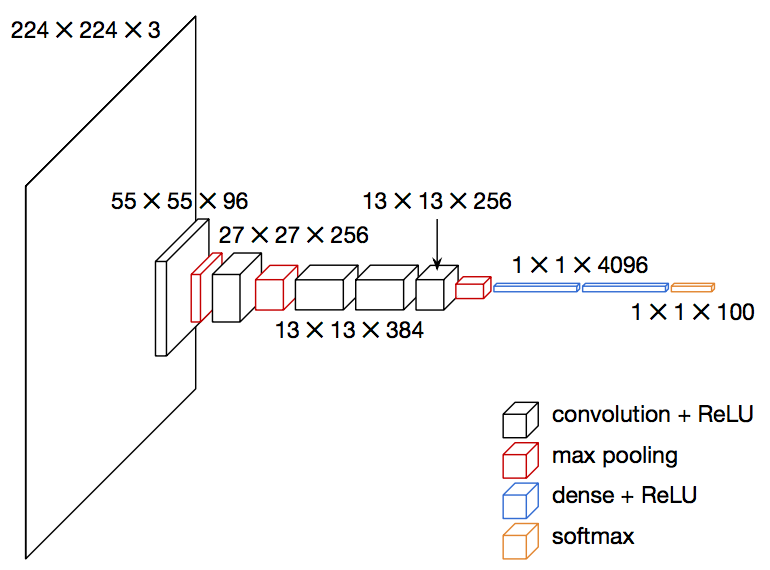
\includegraphics[width=.95\linewidth]{imgs/alexnet.png}
\caption{AlexNet network architecture.}
\label{fig:alexnet}
\end{minipage}%
\begin{minipage}{.58\linewidth}
\centering
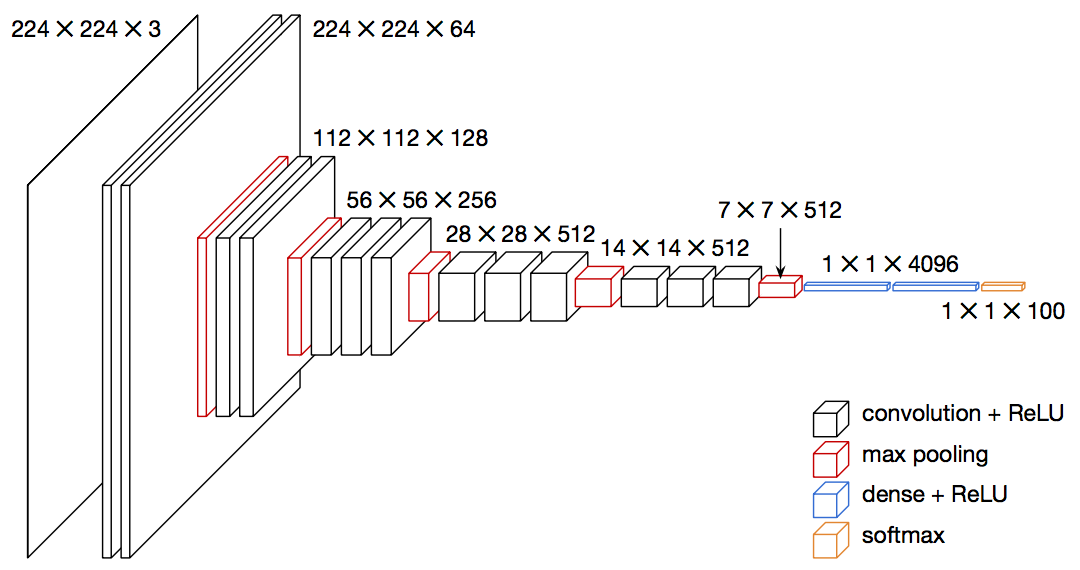
\includegraphics[width=.95\linewidth]{imgs/vgg16.png}
\caption{VGG16 network architecture.}
\label{fig:vgg16}
\end{minipage}
\end{figure*}

\begin{figure*}[ht]
\centering
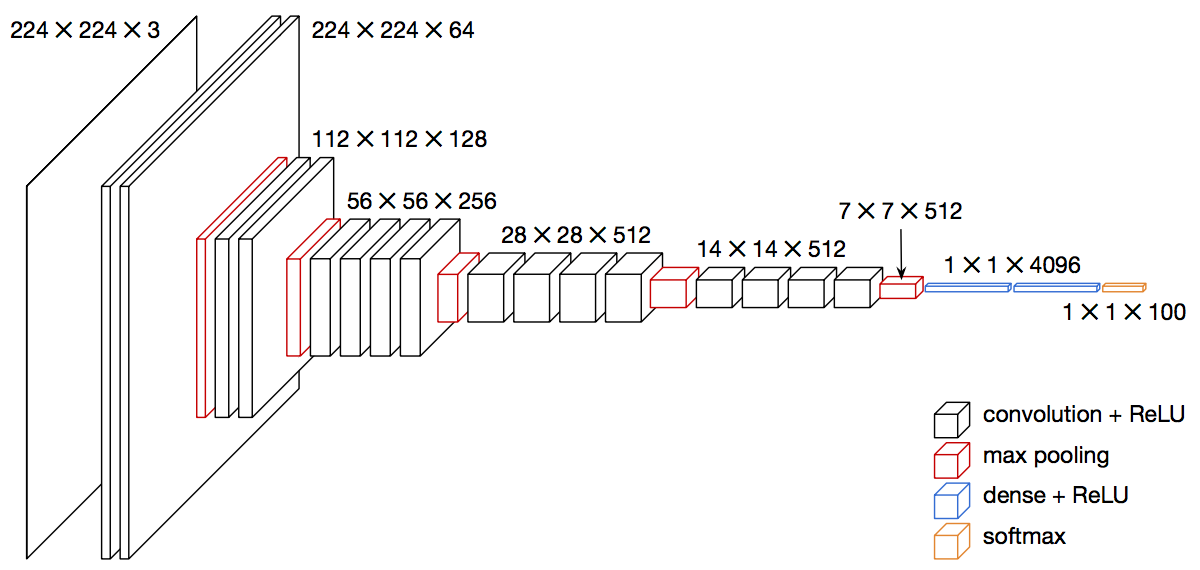
\includegraphics[width=.62\linewidth]{imgs/vgg19.png}
\caption{VGG19 network architecture.}
\label{fig:vgg19}
\end{figure*}

\subsection{AlexNet}
To establish a baseline and ensure that our pipeline is functional, we first implemented AlexNet in Keras.

The network architecture of AlexNet is illustrated in Figure~\ref{fig:alexnet}. The model takes as input a 224 $\times$ 224 $\times$ 3 image. The first convolutional layer filters the input using 96 11 $\times$ 11 kernels and a stride of 4. The second convolutional layer applies 256 5 $\times$ 5 kernels with a stride of 1. The last three convolutional layers apply 3 $\times$ 3 kernels with strides of 1. All max pooling layers operate over a 3 $\times$ 3 window with stride 2. Finally, the network has two fully connected layers with 4096 neurons each. There is a dropout layer with dropout probability 0.5 after each dense layer. The output of the model produces a softmax distribution representing probabilities for each of the 100 scene categories.

In the original implementation of AlexNet, batch normalization is not used. In order to speed up learning and increase overall accuracy~\cite{batchnorm}, we added batch normalization layers after each convolutional and fully connected layer, but before activation layers. This prevented internal covariate shift by ensuring that data between layers are normalized.

\subsection{VGG16}

After implementing AlexNet, we wanted to investigate how increasing the depth of the network would affect the accuracy of the model. Rather than blindly adding convolutional layers to AlexNet, we chose to start with a deep network that was already well-established. VGG16, with twice the number of layers as AlexNet, seemed to be a reasonable model to explore.

The network architecture of VGG16 is illustrated in Figure~\ref{fig:vgg16}. Like AlexNet, the model takes as input a 224 $\times$ 224 $\times$ 3 image. However, unlike AlexNet, all 13 convolutional layers have the same kernel size: 3 $\times$ 3 with strides of 1. All max pooling layers operate over a 2 $\times$ 2 window with stride 2. Finally, as with AlexNet, the network has two fully connected layers with 4096 neurons, each followed by a dropout layer. The output is again passed through a softmax activation to calculate the probability of each of the 100 labels.

The original implementation of VGG16 also does not use batch normalization. Again, to ensure that training occurs in a reasonable period of time, we added batch normalization layers between every convolutional and fully connected layer and their corresponding activation layer.

\subsection{VGG19}

Finally, to further increase the depth of our network, we implemented a version of VGG19 with batch normalization. We added an additional convolutional layer at the third, fourth, and fifth level of convolutional layers, each with the same 3 $\times$ 3 kernels with strides of 1. The network architecture of VGG19 is illustrated in Figure~\ref{fig:vgg19}.

\subsection{Augmenting Dataset}

As the training dataset only contains 100,000 images, we investigated methods to augment our dataset. We primarily explored two methods: image subsampling and horizonally flipping.

To ensure that the model never sees the same exact image twice, we randomly sampled a portion of each image and used the sample to train the model (Figure~\ref{fig:sample}). Specifically, we enlarged the original 128 $\times$ 128 image to a size of 256 $\times$ 256. Then, we randomly selected a 224 $\times$ 224 window within the enlarged image and only included those pixels in the training batch. Thus, the model is more versatile to content appearing at different positions in the image.

In order to match the 224 $\times$ 224 input size, validation and test images are similarly scaled to 256 $\times$ 256. Then. the center 224 $\times$ 224 pixels of the scaled images are used to validate/predict labels.

\begin{figure}[ht]
\centering
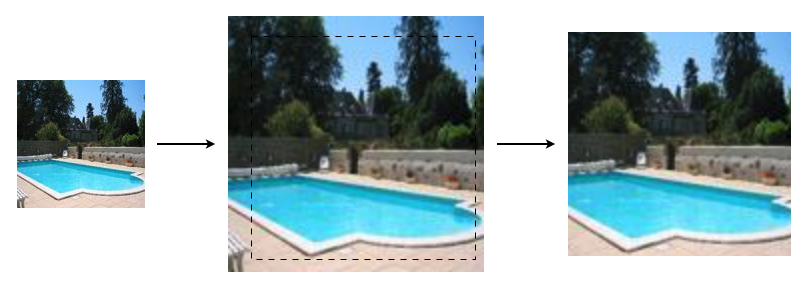
\includegraphics[width=\linewidth]{imgs/sample.png}
\caption{Subsampling images.}
\label{fig:sample}
\end{figure}

Since the content of the images in the dataset are oriented top down, we chose to also augment our dataset by flipping some samples across their vertical axis. For example, the image in Figure~\ref{fig:flip} can still be labeled as a swimming pool regardless if it is mirrored. This also increases the robustness of our model as it is less sensitive to content appearing in different orientations.

\begin{figure}[ht]
\centering
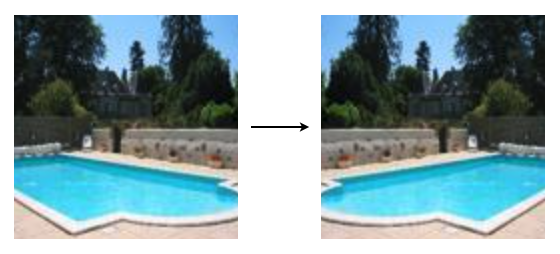
\includegraphics[width=.7\linewidth]{imgs/flip.png}
\caption{Flipping images.}
\label{fig:flip}
\end{figure}

\subsection{Combining Models}\label{sec:combining}

We hypothesize that the features that AlexNet and VGG extract are likely very different since their architectures are so distinct. Thus, it is possible for each model to excel at classifying different images. We predict that we can leverage the strengths of each model by averaging the output predictions from the models.

\subsection{Additional Modifications}\label{sec:additional}

We also tried to explore some ideas from GoogLeNet and ResNet. Specifically, we implemented versions of the GoogLeNet inception module, which applies filters of varying sizes and concatenates the result, and the ResNet residual block, which allows for layers to be effectively ``shorted.'' However, we ran out of both time and computational resources to fully explore the benefits of including these modules in our implementation.


\section{Experiments}

In this section, we provide the results from training and evaluating the various models described in Section~\ref{sec:approach}. As the calculation of test accuracy was rate-limited, we used top-5 validation accuracy as our metric for comparing models.

{\renewcommand{\arraystretch}{1.25}%
\begin{table*}[ht]
\begin{center}
\begin{tabular}{ | c | c | c | c | }
\hline
Base Model & Batch Normalization & Data Augmentation & Top-5 Validation Accuracy \\
\hline\hline
\multirow{4}{*}{AlexNet} &  &  & 0.046 \\
\cline{3-4}
&  & \ding{51} & 0.054 \\
\cline{2-4}
& \multirow{2}{*}{\ding{51}} &  & 0.661 \\
\cline{3-4}
&  & \ding{51} & 0.695 \\
\hline
\multirow{4}{*}{VGG16} &  &  & 0.051 \\
\cline{3-4}
&  & \ding{51} & 0.053 \\
\cline{2-4}
& \multirow{2}{*}{\ding{51}} &  & 0.684 \\
\cline{3-4}
&  & \ding{51} & 0.723 \\
\hline
\multirow{4}{*}{VGG19} &  &  & - \\
\cline{3-4}
&  & \ding{51} & - \\
\cline{2-4}
& \multirow{2}{*}{\ding{51}} &  & 0.707 \\
\cline{3-4}
&  & \ding{51} & 0.739 \\
\hline
\end{tabular}
\end{center}
\caption{Top-5 validation accuracies for combinations of network architecture, batch normalization, and data augmentation.}
\label{table:accuracies}
\end{table*}
}

\subsection{Single Model}

All models were trained with a batch size of 25 and a learning rate of 0.0001. AlexNet models were trained for 24 epochs, while VGG models were trained for 12. All layers have weights initialized according to Xavier initialization and bias initialized to zero.

Table~\ref{table:accuracies} displays the top-5 validation accuracies for various models. Models differ in their base architecture, whether they utilize batch normalization, and whether they use augmented data (subsampling and flipping).

We immediately see that the models without batch normalization essentially did not train. Their performance closely resembles random guessing, as a randomly generated prediction will be correct 5\% of the time. Clearly, in our case, batch normalization was extremely important in order to ensure learning occurs within a reasonable period of time. After we implemented VGG19, we did not test a model without batch normalization.

In addition, for models using batch normalization, augmenting the data increased the accuracies, as expected. On average, the two data augmentation tasks improved top-5 accuracy by around 3 or 4\%.

\subsection{Combining Models}

As discussed in Section~\ref{sec:combining}, we tested if averaging the output predictions from our best AlexNet model and our best VGG model could effectively combine the ``best'' predictions from each of the two models. Table~\ref{table:combining} displays the top-5 validation accuracies for our AlexNet model with batch normalization and augmented data, our VGG19 model with batch normalization and augmented data, and the combined average prediction of the two.

{\renewcommand{\arraystretch}{1.25}%
\begin{table}[ht]
\begin{center}
\begin{tabular}{ | c | c | }
\hline
Model & Top-5 Validation Accuracy \\
\hline\hline
AlexNet & 0.695 \\
VGG19 & 0.739 \\
Combined & 0.752 \\
\hline
\end{tabular}
\end{center}
\caption{Top-5 validation accuracies for our best AlexNet model, VGG19 model, and the combined average prediction of the two models.}
\label{table:combining}
\end{table}
}

Interestingly, while the combined prediction performs better than either of the models by themselves, it only increases accuracy by about 1\%. However, this hybrid model that implements batch normalization, uses augmented data, and combines the results from both an AlexNet and VGG19 network, yields a 70\% increase in top-5 accuracy compared to the baseline AlexNet model we started with. When used to predict labels for the test images, this hybrid model achieves a top-5 accuracy of 0.752.

\subsection{Future Work}

Given more time, we would have liked to explore a few more approaches. If we had more computational resources, we would have wanted to explore how including both inception modules and residual blocks in our models could have improved their performance, as stated in Section~\ref{sec:additional}. In addition, we would have liked to experiment with additional data augmentations, including randomly rotating and zooming the images. It would also be interesting to see if adding random noise to images, or even combining two images together, could improve the accuracy of our predictions.


{\small
\bibliographystyle{ieee}
\bibliography{bib}
}

\end{document}
